\documentclass[a4paper,12pt]{article}

\usepackage[margin=2.5cm]{geometry}
\usepackage{lipsum}
\usepackage{libertine}
\usepackage{multirow}
\usepackage{makecell}
\usepackage{tabularx}
\usepackage{graphicx}
\usepackage{soul}
\usepackage{xcolor}
\usepackage{booktabs}
\usepackage{amsmath}
\usepackage[colorlinks=false, pdfborderstyle={/S/U/W 1}]{hyperref}

\usepackage{fontspec}
\setmonofont{Courier New}

\usepackage[backend=biber, 
natbib=true, 
style=C:/texmf/bst/biblatex-sp-unified/bbx/biblatex-sp-unified,
citestyle=C:/texmf/bst/biblatex-sp-unified/cbx/sp-authoryear-comp, 
maxbibnames=99, 
isbn=false, 
doi=false, 
eprint=false]{biblatex}
\addbibresource{qp.bib}

\usepackage[libertine]{newtxmath} % to get libertine as math font too

\usepackage{xspace}

\usepackage{enumitem}
%\setlist{nosep}
\setlist{noitemsep}

\usepackage{url}
%\urlstyle{same}

\usepackage{setspace}
\onehalfspacing

%\pagenumbering{gobble}

% ------------------------------------------------------------------------------------------------------ %

\begin{document}

\noindent PM1 Question Processing \hfill \today

\vspace{-\baselineskip}

\section*{Project plan: 20 Questions}
\noindent Wellesley Boboc, Anna-Janina Goecke, Rodrigo Lopez Portillo Alcocer, Elizabeth Pankratz

\subsection*{Task and motivation}

Our task is to build a system that will play the game 20 Questions (20Q).
A human player will be able to think of a target object, and the system will strategically select questions that allow it to narrow down the candidate objects in its knowledge base.
It will incorporate the answers it receives and ultimately make a guess about what that target object could be.
If the target object that the human player has in mind is not already in its knowledge base, the system will add it in based on the information the user has provided.

This task is interesting and challenging, because it not only involves generating natural-language questions to present to the human player, but also choosing which questions are the best ones to ask, and manipulating the knowledge representation in accordance with the answers that the human player provides.

So, on the one hand, the project contains the computational-linguistic subtask of question generation (given a feature in the dataset, generate a natural-language question asking about that feature to display to the user), and on the other, the engineering subtask of knowledge base manipulation.
There, we will need to strategically select the best question to ask, incorporate the answers from the user as the game is played, and at the end, add previously-unseen objects into the knowledge base.

\subsection*{Related work}

\hl{TODO: What work are you building on (= papers you read)?  What have they done? How do they define the problem? Is this a good kind of definition? What do you approach differently from them / how do you go beyond?}

We could take inspiration from literature on 20Q overall (there have been RL approaches, what else?) as well as from literature on rule-based question generation.

\subsection*{Data}
We are currently developing the implementation on a preliminary knowledge set available \href{https://github.com/drdevinhopkins/20_Questions/blob/master/knowledge_base.csv}{here}.
It is a table consisting of 100 objects (mostly animals) and 28 features for each, and each cell in the table is populated with a 1 or a 0 to indicate that the given animal does or does not have the given feature.
For example, the first few rows and columns of the dataset look like this:

\begin{center}
	\begin{tabular}{lcccccc}
	\toprule
Animal & Hair & Feathers & Eggs & Milk & Airborne & \ldots \\ \midrule
aardvark & 1 & 0 & 0 & 1 & 0 & \ldots \\
antelope & 1 & 0 & 0 & 1 & 0 & \ldots \\
bass & 0 & 0 & 1 & 0 & 0 & \ldots \\
bear & 1 & 0 & 0 & 1 & 0 & \ldots \\
boar & 1 & 0 & 0 & 1 & 0 & \ldots \\
\vdots & \vdots & \vdots & \vdots & \vdots & \vdots & $\ddots$ \\
\bottomrule
\end{tabular}
\end{center}

Whichever dataset we end up actually using should be larger than this and have many more features, since the system is currently almost always able to finish within the 20-question limit.
We are currently looking for open-source knowledge bases like this to use.

\subsection*{Implementation}

The machine learning system that we will use to implement this task is fairly simple: a decision tree (DT), also known as a CART model, which stands for ``classification and regression tree'' \citep[Section 16.2]{Murphy2012}.
A DT is ``defined by recursively partitioning the input space, and defining a local model in each resulting region of input space'' \citep[545]{Murphy2012}.
In our case, the input space consists of the knowledge base described above, and this knowledge base is recursively partitioned by each successive question that the system asks and the user answers.
However, in contrast to defining a local model in \textit{each} resulting region of input space, we will only retain the subset of the knowledge base that is compatible with the user's answers.

But how will we partition the space in an optimal way, or in other words, how will we choose which question to ask?
One standard method in classification DTs splits the space on the feature that minimises the entropy (i.e.\ maximises the information gain; \citealt{Quinlan1986}), in each partition.
However, that method is not applicable here.
That method requires an $n : 1$ mapping of instances to each class, which is the usual set-up in classification problems: one class contains multiple instances.
In our task, though, each individual object equates to a class (i.e.\ there's an \textit{aardvark} class, an \textit{antelope} class, and so on), so there is only one instance per class.
That makes our problem a non-typical classification task, so a different method needs to be used.

We chose to orient ourselves around the size of the two partitions of the input space that result from splitting on a given feature, and we select the feature that produces the partitions that are closest to each other in size.
To illustrate, say that we split on the first feature given above, \textit{Hair}.
We would end up with one partition containing 57 animals that have no hair (i.e.\ where \textit{Hair} $= 0$), and another partition containing 43 animals with hair (i.e.\ where \textit{Hair} $= 1$).
To see how even this split is, we take a ratio of these two numbers.
We want this ratio to be as close to 1 as possible, since that would represent a perfect split of our input space in half: $\frac{50}{50} = 1$.
This is because since we only have two ``branches" for each feature (yes or no, 1 or 0), consistently splitting our input space in half would result in the highest information gain regarding the class label. We selected this approach based on tree-based algorithms such as ID3.

So, for the feature \textit{Hair}, we get

$$\frac{|Hair = 0|}{|Hair = 1|} = \frac{57}{43} \approx 1.33.$$

We call this value, $1.33$, the \textsc{split cardinality ratio} (SCR) for the feature \textit{Hair}, and we want to choose the feature whose SCR is as close as possible to 1.
Or in other words, we want to choose the feature $f$ for which $abs(1 - SCR(f))$ is minimised.
We illustrate this principle by also looking at the feature that actually minimises  $abs(1 - SCR(f))$ in the current development dataset, \textit{Predator}:

\begin{align*}
\frac{|Predator = 0|}{|Predator = 1|} &= \frac{45}{55} \approx 0.82 \\
\implies SCR(Predator) & = 0.82\\
\implies abs(1 - SCR(Predator)) &= 0.18.
\end{align*}

For \textit{Hair}, this value is $abs(1 - 1.33) = 0.33$, which is greater than $0.18$, so given the choice between these two features, our system would choose to split the input space on \textit{Predator} rather than \textit{Hair}.
In question-processing terms, this means we would ask the user a question like ``Is it a predator?'' rather than ``Does it have hair?".

So in this way, for each question the system has to ask, we compute the SCRs of all features in the input space, and choose the one with the smallest value of $abs(1 - SCR)$ (or if there are multiple features with the same value, we randomly choose between them).
The first split of the development dataset is always on \textit{Predator}, since that results in the most even partition of the input space into subsets of size 45 or 55, depending on whether the user answers 0 or 1.
%(Then eventually, if none of the features contain mixtures of 0s and 1s and thus cannot be used to distinguish objects anymore, we switch to cycling through all candidate objects that cannot be further differentiated and asking about each of them in turn.)

There are certainly other strategies that could be used for choosing a question.
This algorithm could be made more sophisticated by learning from previous games, or by performing an analysis of the features to see which ones are mutually exclusive, and so on.
But we're keeping it simple for now.

The steps in our implementation will be as follows (everything following 1 can be concurrent):
\begin{enumerate}
	\item Write baseline DT system that decides at each step the optimal question to ask, narrows down the knowledge base to the objects compatible with the yes/no answers it receives, and ultimately makes guesses until the number of questions has reached 20 (we've pretty much finished this already).
	\item Incorporate handling of answers beyond yes and no.
	\item Implement the rule-based question generation, based on the structures of yes/no questions in corpora, e.g.\ Switchboard.
	\item Implement the incorporation of previously-unseen objects into the knowledge base.
\end{enumerate}

\subsection*{Evaluation}

There is a straightforward measure of success of our system overall: $\frac{\text{games won}}{\text{games played}}$. But because the system will consistently improve as we add new objects to its knowledge base, the success rates we get in early games with the system will presumably not be as good as success rates from later games. We can track this in a sort of growth curve across games:
	
\begin{center}
	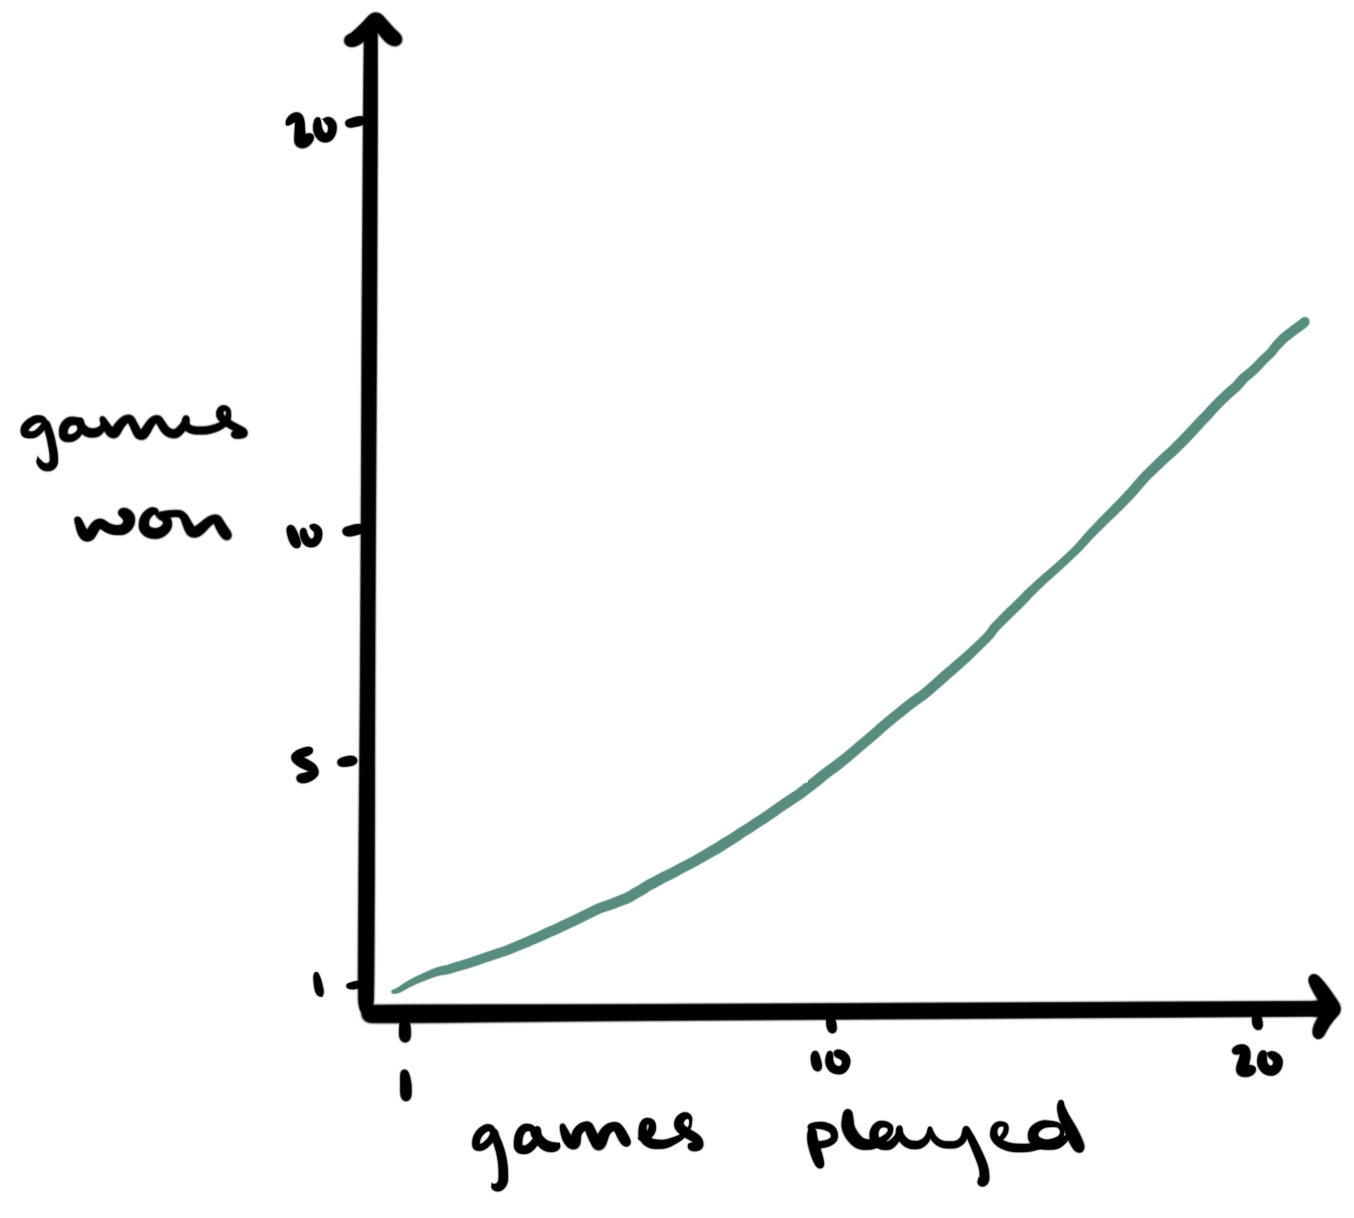
\includegraphics[width=.5\linewidth]{growth-curve.png}
\end{center}

The slope of the curve won't ever get bigger than one, but we'd want it to approach one, since that means the system is winning every game that it plays.
The slope of that curve at its endpoint is actually given by the rational expression $\frac{\text{games won}}{\text{games played}}$ \citep[50--51]{Baayen2001}, so we can evaluate how our system performs after $x$ games by looking at how close that value is to one.
Or alternately, we could look at $\frac{\text{games lost}}{\text{games played}}$ and see how close that value is to zero.
\begin{center}
	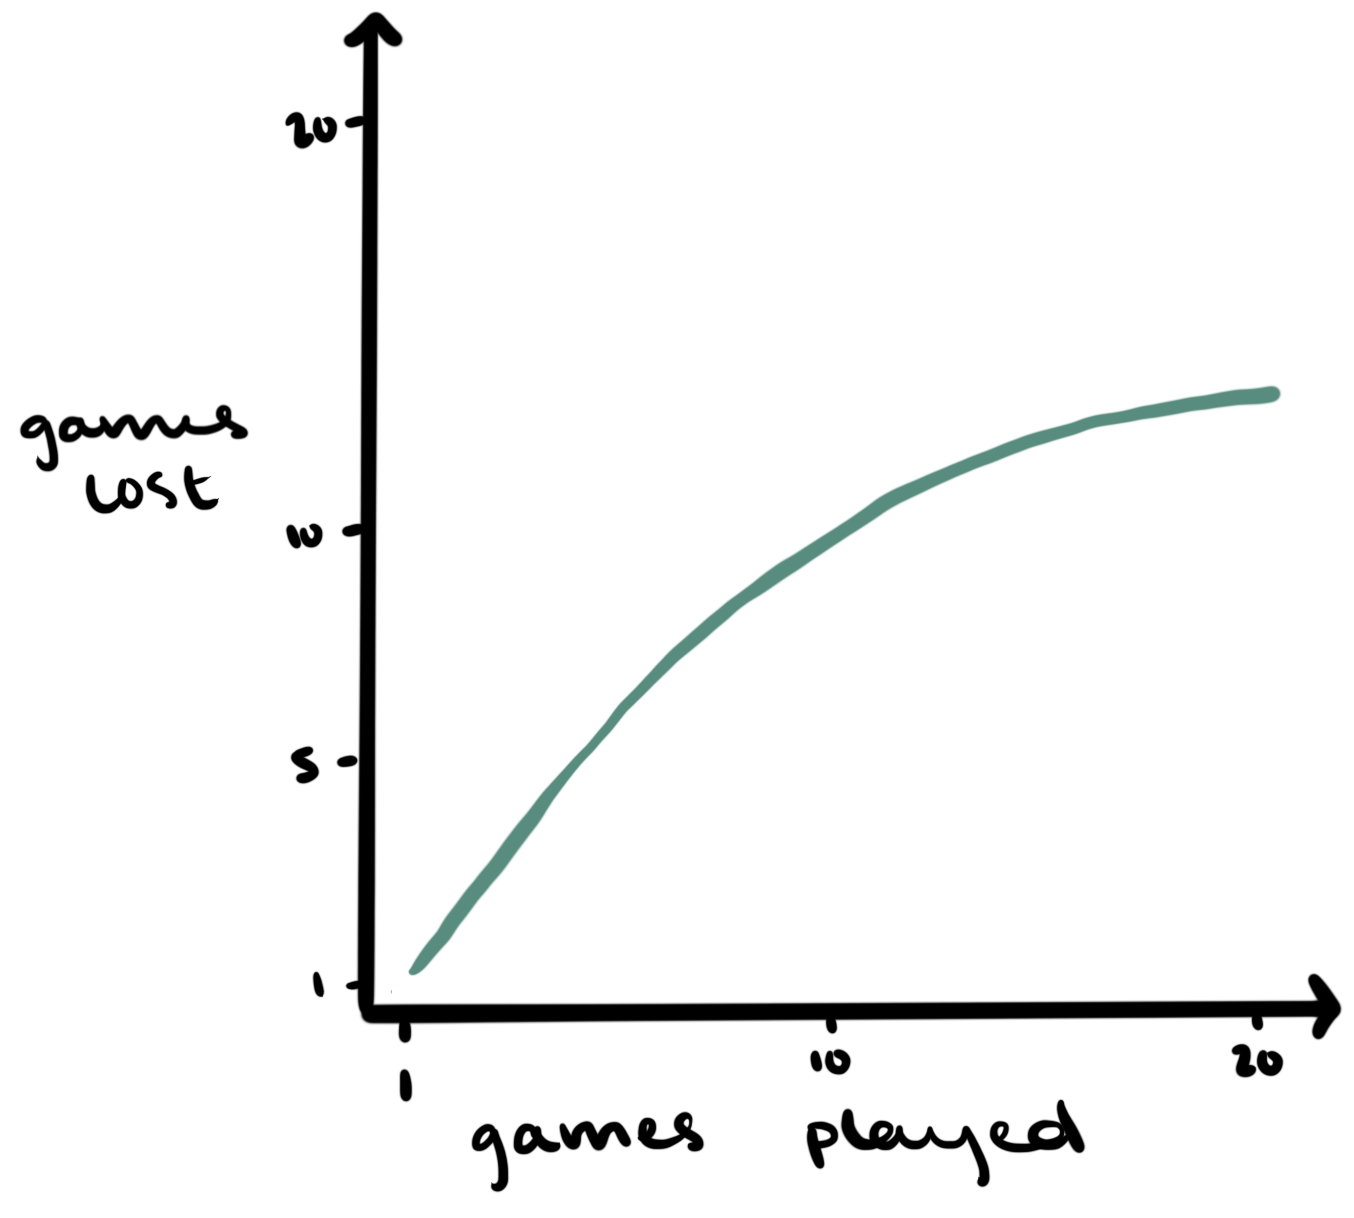
\includegraphics[width=.5\linewidth]{growth-curve2.png}
\end{center}

Depending on how intense we want to get about this whole thing, we could model this second growth curve using a Zipf-Mandelbrot model \citep{Evert2004}, and that would allow us to predict how many games our system would have lost after an arbitrarily large number of games played.
There is a package in R that we could use to do this: \texttt{zipfR} by \citet{BaroniEvert2014}.

(We should also keep track of whether/how many losses come from exceeding the 20 question limit and how many come from out-of-database items. Ideally, the 20-question-limit curve will not change much, and the out-of-database curve would change more.
Wellesley also mentioned that we should count the number of questions that it takes for the system to win.)

Also, we should evaluate the goodness of the out-of-database items that we interpolate.
We could use human annotators who don't look at any of the other items in the dataset and only annotate the out-of-database items for all the features we use? 
Then we can compare their results to those output by Rodrigo's system. 
(We could either do it ourselves or source some ``crowdworkers'' among our friends using Google Forms again---will leave this up to Anna and/or Wellesley).

% -----------------------------------------------
\singlespacing
\printbibliography
% -----------------------------------------------

\end{document}